\documentclass[11pt,letterpaper]{article}

\usepackage[margin=1in,headheight=14pt]{geometry}
\usepackage{amsmath,amssymb,amsthm,mathtools}
\usepackage{graphicx}
\usepackage{xcolor}
\usepackage{enumitem}
\usepackage{microtype}
\usepackage{fancyhdr}
\usepackage[colorlinks=true,linkcolor=blue,citecolor=blue,urlcolor=blue]{hyperref}

% Personal notation and theorem environments.
%!TEX root = EM_singular_models.tex

% PDF margin etc settings
%\setlength{\textwidth}{\paperwidth}
%\addtolength{\textwidth}{-6cm}
%\setlength{\textheight}{\paperheight}
%\addtolength{\textheight}{-4cm}
%\addtolength{\textheight}{-1.1\headheight}
%\addtolength{\textheight}{-\headsep}
%\addtolength{\textheight}{-\footskip}
%\setlength{\oddsidemargin}{0.5cm}
%\setlength{\evensidemargin}{0.5cm}

%%%%%%%%%%%%%%%%%%%%%%%%%%%%%%%%

% MACROS HERE

%%%%%%%%%%%%%%%%%%%%%%%%%%%%%%%%

\newcommand{\fixedpointtheta}{\widehat\theta_\obs}

\newcommand{\cover}{N}
\newcommand{\kinit}{\nu}
\newcommand{\cdelta}{c_\threshold}
\newcommand{\dndelta}{\omega}
\newcommand{\kndelta}{\Upsilon}
\newcommand{\kndeltanew}{\Psi}
\newcommand{\radii}{\mathcal{R}}
\newcommand{\event}{\mathcal{E}}
\newcommand{\kevent}{\mathcal{D}}


% Observations, dimension etc.
\newcommand{\dims}{\ensuremath{d}}
\newcommand{\samples}{\ensuremath{n}}
\newcommand{\obs}{\samples}
\newcommand{\real}{\ensuremath{\mathbb{R}}}
\newcommand{\complex}{\ensuremath{\mathbb{C}}}
\newcommand{\realdim}{\ensuremath{\real^\dims}}

\newcommand{\smallthreshold}{\epsilon}

% some mathcal notations
\newcommand{\order}[1]{\ensuremath{\mathcal{O}\parenth{#1}}}

% Basic statistics notation
\newcommand{\xstar}{\ensuremath{x^*}}
\newcommand{\xbar}{\ensuremath{\bar{x}}}
% True parameter
\newcommand{\thetastar}{\ensuremath{{\theta^*}}}
% Estimate one
\newcommand{\thetahat}{\ensuremath{\widehat{\theta}}}
% Estimate two
\newcommand{\thetatil}{\ensuremath{\widetilde{\theta}}}
\newcommand{\thetabar}{\ensuremath{\bar{\theta}}}
\newcommand{\yvec}{\ensuremath{y}}
\newcommand{\Xmat}{\ensuremath{X}}

% Distributions
\newcommand{\distribution}{P}
\newcommand{\density}{f}
\newcommand{\gaussiandensity}{\phi}
\newcommand{\NORMAL}{\ensuremath{\mathcal{N}}}
\newcommand{\BER}{\ensuremath{\mbox{Ber}}}

% Spaces
\newcommand{\Xspace}{\ensuremath{\mathcal{X}}}
\newcommand{\Yspace}{\ensuremath{\mathcal{Y}}}
\newcommand{\Zspace}{\ensuremath{\mathcal{Z}}}


% Brackets Size
\newcommand{\brackets}[1]{\left[ #1 \right]}
\newcommand{\parenth}[1]{\left( #1 \right)}
\newcommand{\bigparenth}[1]{\big( #1 \big)}
\newcommand{\biggparenth}[1]{\bigg( #1 \bigg)}
\newcommand{\braces}[1]{\left\{ #1 \right \}}
\newcommand{\abss}[1]{\left| #1 \right |}
\newcommand{\angles}[1]{\left\langle #1 \right \rangle}
\newcommand{\tp}{^\top}

% Generic vectors and scalars
\newcommand{\myvec}{u} % for generic vector
\newcommand{\myvectwo}{v} % for generic vector
\newcommand{\mymat}{B}
\newcommand{\set}{{A}}
\newcommand{\scalar}{\alpha}
\newcommand{\tvscalar}{\epsilon}
\newcommand{\tailboundscalar}{t}
\newcommand{\term}{U}
\newcommand{\myVarone}{\alpha_X}
\newcommand{\myVartwo}{\alpha_Y}
\newcommand{\myCovmat}{\Sigma}
\newcommand{\xcord}[1]{x^{(#1)}}
\newcommand{\xcordpop}[1]{X^{(#1)}}
\newcommand{\ycordpop}[1]{Y^{(#1)}}
\newcommand{\myVarthree}{\ensuremath{U}}
\newcommand{\myVarfour}{\ensuremath{V}}
\newcommand{\myfuntwo}{\ensuremath{g}}
\newcommand{\numsteps}{t}
\newcommand{\totalnumsteps}{T}
\newcommand{\seqalpha}[1]{\alpha_{#1}}
\newcommand{\seqnu}[1]{\nu^{(#1)}}
\newcommand{\imax}{\ell_\smallthreshold}
\newcommand{\basis}{e}
\newcommand{\radem}{\varepsilon}
\newcommand{\Tone}{T\ensuremath{_{0}}}
\newcommand{\Ttwo}{T\ensuremath{_{2}}}
\newcommand{\contractPar}[1]{\ensuremath{\gamma\parenth{#1}}}

\newcommand{\simiid}{\overset{\mathrm{i.i.d.}}{\sim}}
\newcommand{\eqd}{\overset{d}{=}}


% EM updates
\newcommand{\hidden}{Z}
\newcommand{\qfun}[2]{Q(#1\vert#2)}
\newcommand{\variable}{\theta}
\newcommand{\weights}{w}
\newcommand{\myfun}{q}
\newcommand{\gradf}{\nabla \myfun}
\newcommand{\hessf}{\nabla^2 \myfun}
\newcommand{\iter}{t}
\newcommand{\mupdate}{M}
\newcommand{\mupdategeneral}{\ensuremath{M^{GN}}}




% EM contractions
\newcommand{\contractgene}{\ensuremath{\gamma^{GN}}}
\newcommand{\updateMat}{\ensuremath{\Gamma_{\theta}}}
\newcommand{\mymatTheta}{\ensuremath{B_{\theta}}}
\newcommand{\sech}{\text{sech}}

% Nhat's macros 
\newcommand{\Rspace}{\ensuremath{\mathbb{R}}}
\newcommand{\Ecal}{\ensuremath{\mathcal{E}}}
\newcommand{\Ncal}{\ensuremath{\mathcal{N}}}
\newcommand{\gradient}{\ensuremath{\nabla}}
\newcommand{\smallweight}{\ensuremath{\epsilon^{sw}}}
\newcommand{\smallnorm}{\ensuremath{\rho^{sw}}}
\newcommand{\ball}{\ensuremath{\mathbb{B}}}
\newcommand{\sphere}{\ensuremath{\mathbb{S}}}

\newcommand{\diam}{\ensuremath{\text{diam}}}
\newcommand{\upper}{\ensuremath{\bar{C}}}
\newcommand{\sample}{\ensuremath{\xi}}
\newcommand{\weight}{\ensuremath{\pi}}
\newcommand{\contracasym}{\ensuremath{\rho}}
\newcommand{\Fishermatrix}{\ensuremath{\mathcal{I}}}
\newcommand{\barcontracasym}{\ensuremath{\bar{\rho}}}


\newcommand{\TrueDensity}{\ensuremath{f}}
\newcommand{\FitDensity}{\ensuremath{f}_{\theta}}
\newcommand{\FitDensityfree}{\ensuremath{f}_{\pi, \theta}}
\newcommand{\FitDensitygen}{\ensuremath{f}_{\pi, \theta_{1}, \theta_{2}}}
\newcommand{\FitDensitymore}{\ensuremath{f}_{G}}
\newcommand{\normden}{\ensuremath{\phi}}
\newcommand{\mean}{\ensuremath{\theta}}
\newcommand{\sd}{\ensuremath{\sigma}}
\newcommand{\parFOS}{\ensuremath{\gamma}}
\newcommand{\funQ}{\ensuremath{Q}}
\newcommand{\updateM}{\ensuremath{M}}
\newcommand{\weightFun}{\ensuremath{w}}
\newcommand{\mydefn}{\ensuremath{:=}}
\newcommand{\poincare}{\ensuremath{\tilde{C}}}
\newcommand{\paraspace}{\ensuremath{\Theta}}
\newcommand{\loglihood}{\ensuremath{F}}
\newcommand{\prior}{\ensuremath{\pi}}
\newcommand{\posterior}{\ensuremath{\Pi}}
\newcommand{\boundcons}{\ensuremath{B}}
\newcommand{\boundconstot}{\ensuremath{H}}
\newcommand{\noise}{\ensuremath{\varepsilon}}
\newcommand{\loglihoodgaus}{\ensuremath{F^{G}}}
\newcommand{\loglihoodind}{\ensuremath{F^{I}}}
\newcommand{\loglihoodlogit}{\ensuremath{F^{R}}}
\newcommand{\noiseone}{\ensuremath{\varepsilon_{1}}}
\newcommand{\noisetwo}{\ensuremath{\varepsilon_{2}}}

%%%SDE_Bayesian_inf
\newcommand{\weakcon}{\ensuremath{\psi}}
\newcommand{\perturb}{\ensuremath{\zeta}}
\newcommand{\inver}{\ensuremath{\xi}}

% Universal constants
\newcommand{\unicon}{c}
\newcommand{\uniconnew}{c'}
\newcommand{\uniconone}{c_1}
\newcommand{\unicontwo}{c_2}

% some parameters that you may define
\newcommand{\scparam}{m} % strong  convexity parameter
\newcommand{\smoothness}{L} % smoothness parameter
\newcommand{\step}{h}


%%%%%%%%% Distributions and Random variables %%%%%%%%%%%
\newcommand{\rvg}{\xi} % to denote the random variable g
\newcommand{\threshold}{\delta}


%%%%%%%%% Basic Terms like defn, etal, tmix, polylog %%%%%%%%%%%
\newcommand{\defn}{:=}
\newcommand{\rdefn}{=:}
\newcommand{\etal}{{et al.}}
\newcommand{\polylog}{\text{poly-log}}

% Some vector/matrix norms
\newcommand{\matnorm}[3]{|\!|\!| #1 | \! | \!|_{{#2}, {#3}}}
\newcommand{\matsnorm}[2]{|\!|\!| #1 | \! | \!|_{{#2}}}
\newcommand{\vecnorm}[2]{\left\| #1\right\|_{#2}}
\newcommand{\enorm}[1]{\vecnorm{#1}{2}} % euclidean norm
\newcommand{\nucnorm}[1]{\ensuremath{\matsnorm{#1}{\footnotesize{\mbox{nuc}}}}}
\newcommand{\fronorm}[1]{\ensuremath{\matsnorm{#1}{\footnotesize{\mbox{fro}}}}}
\newcommand{\opnorm}[1]{\ensuremath{\matsnorm{#1}{\tiny{\mbox{op}}}}}
%%% EM paper
\newcommand{\constrainnorm}[1]{\vecnorm{#1}{[k]}} % euclidean norm

\newcommand{\bigmatsnorm}[2]{{\Big|\!\Big|\!\Big| #1
  \Big|\!\Big|\!\Big|}_{#2}}

% Inner product
\newcommand{\inprod}[2]{\ensuremath{\langle #1 , \, #2 \rangle}}

% Kullback-Leibler
\newcommand{\kull}[2]{\ensuremath{D_{\text{KL}}(#1\; \| \; #2)}}

% Probability
\newcommand{\Exs}{\ensuremath{{\mathbb{E}}}}
\newcommand{\Prob}{\ensuremath{{\mathbb{P}}}}

%Eigenvector / eigenvalue related notation
\newcommand{\eig}[1]{\ensuremath{\lambda_{#1}}}
\newcommand{\eigmax}{\ensuremath{\eig{\max}}}
\newcommand{\eigmin}{\ensuremath{\eig{\min}}}

% \DeclareMathOperator{\det}{det}
\DeclareMathOperator{\modd}{mod}
\DeclareMathOperator{\diag}{diag}
\DeclareMathOperator{\var}{var}
\DeclareMathOperator{\cov}{cov}
\DeclareMathOperator{\trace}{trace}
\DeclareMathOperator{\abs}{abs}
\DeclareMathOperator{\floor}{floor}
\DeclareMathOperator{\vol}{vol}
\DeclareMathOperator{\child}{child}
\DeclareMathOperator{\parent}{parent}
\DeclareMathOperator{\sign}{sign}
\DeclareMathOperator{\rank}{rank}
\DeclareMathOperator{\toeplitz}{toeplitz}




\newtheoremstyle{named}{}{}{\itshape}{}{\bfseries}{.}{.5em}{\thmnote{#3's }#1}
\theoremstyle{named}
\newtheorem*{namedtheorem}{Lemma}

%%%%%%%
\theoremstyle{plain}

% {Theorem, Proposition, Lemma, Corollary} numbered sequentially
% throughout the paper
\newtheorem{theorem}{Theorem}
\newtheorem{proposition}{Proposition}
\newtheorem{lemma}{Lemma}
\newtheorem{claim}{Claim}
\newtheorem{corollary}{Corollary}
\newtheorem{definition}{Definition}
\newtheorem{conjecture}{Conjecture}
\newtheorem{remark}{Remark}
%%%%%%%%%%%%%%%%%%%%%%%%%%%%%%%%%%%%%%%%%%%%%%%%%%%%%%%%%%%%%%%%%%%%%%%
% WIDEBAR COMMAND
\newlength{\widebarargwidth}
\newlength{\widebarargheight}
\newlength{\widebarargdepth}
\DeclareRobustCommand{\widebar}[1]{%
  \settowidth{\widebarargwidth}{\ensuremath{#1}}%
  \settoheight{\widebarargheight}{\ensuremath{#1}}%
  \settodepth{\widebarargdepth}{\ensuremath{#1}}%
  \addtolength{\widebarargwidth}{-0.3\widebarargheight}%
  \addtolength{\widebarargwidth}{-0.3\widebarargdepth}%
  \makebox[0pt][l]{\hspace{0.3\widebarargheight}%
    \hspace{0.3\widebarargdepth}%
    \addtolength{\widebarargheight}{0.3ex}%
    \rule[\widebarargheight]{0.95\widebarargwidth}{0.1ex}}%
  {#1}}



%%% New version of \caption puts things in smaller type, single-spaced
%%% and indents them to set them off more from the text.
\makeatletter
\long\def\@makecaption#1#2{
        \vskip 0.8ex
        \setbox\@tempboxa\hbox{\small {\bf #1:} #2}
        \parindent 1.5em  %% How can we use the global value of this???
        \dimen0=\hsize
        \advance\dimen0 by -3em
        \ifdim \wd\@tempboxa >\dimen0
                \hbox to \hsize{
                        \parindent 0em
                        \hfil
                        \parbox{\dimen0}{\def\baselinestretch{0.96}\small
                                {\bf #1.} #2
                                %%\unhbox\@tempboxa
                                }
                        \hfil}
        \else \hbox to \hsize{\hfil \box\@tempboxa \hfil}
        \fi
        }
\makeatother



%% COMMENTING commands

\long\def\comment#1{}
\definecolor{battleshipgrey}{rgb}{0.52, 0.52, 0.51}
\definecolor{darkgray}{rgb}{0.66, 0.66, 0.66}
\definecolor{darkgreen}{rgb}{0.0, 0.2, 0.13}
\definecolor{darkspringgreen}{rgb}{0.09, 0.45, 0.27}
\definecolor{dukeblue}{rgb}{0.0, 0.0, 0.61}
\definecolor{olivedrab7}{rgb}{0.24, 0.2, 0.12}
\definecolor{darkblue}{rgb}{0.0, 0.0, 0.55}
\definecolor{darkscarlet}{rgb}{0.34, 0.01, 0.1}
\definecolor{candyapplered}{rgb}{1.0, 0.03, 0.0}
\definecolor{ao(english)}{rgb}{0.0, 0.5, 0.0}
\definecolor{applegreen}{rgb}{0.55, 0.71, 0.0}

\newcommand{\red}[1]{\textcolor{red}{#1}}
\newcommand{\mjwcomment}[1]{{\bf{{\red{{MJW --- #1}}}}}}
\newcommand{\mwlcomment}[1]{{\bf{{\color{orange}{{Wenlong --- #1}}}}}}

\newcommand{\blue}[1]{\textcolor{blue}{#1}}
\newcommand{\green}[1]{\textcolor{green}{#1}}
\newcommand{\highlight}[1]{\textcolor{applegreen}{#1}}

% comment lines
\newcommand{\genecomment}[1]{{\bf{{\blue{{TEAM --- #1}}}}}}
\newcommand{\rrdcomment}[1]{{\bf{{\blue{{RRD --- #1}}}}}}
\newcommand{\nhcomment}[1]{{\bf{{\blue{{NH --- #1}}}}}}
\newcommand{\kkcomment}[1]{{\bf{{\darkgreen{{KK --- #1}}}}}}


\newcommand{\widgraph}[2]{\includegraphics[keepaspectratio,width=#1]{#2}}


\newcommand{\coursenumber}{STA3000F}
\newcommand{\coursetitle}{Advanced Theory of Statistics}
\newcommand{\courseterm}{Fall 2026}
\newcounter{lecture}
\setcounter{lecture}{3}
\newcommand{\lecturenumber}{\arabic{lecture}}
\newcommand{\lecturedate}{September 25, 2026}
\newcommand{\lecturer}{Wenlong Mou}

\pagestyle{fancy}
\fancyhf{}
\fancyhead[L]{\coursenumber: \coursetitle}
\fancyhead[R]{Lecture \lecturenumber}
\fancyfoot[C]{\lecturenumber--\arabic{page}}
\renewcommand{\headrulewidth}{0.4pt}
\renewcommand{\footrulewidth}{0pt}

\usepackage{bm}

\renewcommand{\thepage}{\lecturenumber--\arabic{page}}

\newtheorem{example}{Example}
\numberwithin{theorem}{lecture}
\numberwithin{proposition}{lecture}
\numberwithin{lemma}{lecture}
\numberwithin{claim}{lecture}
\numberwithin{corollary}{lecture}
\numberwithin{definition}{lecture}
\numberwithin{conjecture}{lecture}
\numberwithin{remark}{lecture}
\numberwithin{example}{lecture}
\numberwithin{equation}{lecture}
\counterwithin*{section}{lecture}
\renewcommand{\theHsection}{\arabic{lecture}.\arabic{section}}

\newcommand{\makelecturenotesheader}{%
  \noindent
  \textbf{\coursenumber: \coursetitle}%
  \hfill
  \textbf{\courseterm}

  \begin{center}
    {\Large\bfseries Lecture \lecturenumber: \lecturedate}
  \end{center}

  \noindent
  \textbf{Lecturer:} \lecturer
  \par\medskip
  \hrule
  \bigskip
}

\begin{document}

\makelecturenotesheader

\section{Sufficiency continued -- UMVUE}
\begin{definition}[Complete statistics]
  We call a statistic $T(X)$ complete if for any measurable function $g$ such that
  \begin{align*}
    \Exs_\theta [g(T(X))] = 0, \quad \forall \theta \in \Theta,
  \end{align*}
  we have $g(T(X)) = 0$ almost surely with respect to $\Prob_\theta$ for all $\theta \in \Theta$.
\end{definition}
Intuition: $g$ does not contain redundant information.
\begin{itemize}
  \item Sufficiency: $T(X)$ contains all information (contained in the data) about $\theta$, but there may be redundant information in $T(X)$.
  \item Completeness is complementary to sufficiency: $T(X)$ may incur loss of information, but on the other hand, if there's some redundancy in $T(X)$, we can find a function $g$ that extracts the redundant information, and then $\Exs_\theta [g(T(X))]$ will not depend on $\theta$.
\end{itemize}
e.g. Let $X_1, X_2, \cdots, X_n \simiid \mathrm{Unif} ([\theta - 1, \theta + 1])$.
\begin{itemize}
  \item For $T (X_1, \cdots, X_n) = (X_1, X_2, \cdots, X_n)$, we can take $g(T) = X_1 - X_2$. Then $\Exs_\theta [g(T)] = 0$ for all $\theta$, but $g(T)$ is not almost surely zero. So $T$ is not complete.
  \item For $T (X_1, \cdots, X_n) = (X_{(1)}, X_{(n)})$, we can show that $T$ is complete. (See Keener's textbook for a proof.)
\end{itemize}
e.g. Let $X_1, X_2, \cdots, X_n \simiid \mathrm{Unif} ([0, \theta])$. Consider the sufficient statistic $T(X_1, \cdots, X_n) = X_{(n)}$. To show that $T$ is complete, we note that
\begin{align*}
  \Prob_\theta (T (X_1, X_2, \cdots, X_n) \leq t) = (t / \theta)^n \quad \text{for } t \in [0, \theta].
\end{align*}
Now that if you have a function $g$ such that $\Exs_\theta [g(T)] = 0$ for all $\theta$, then we have
\begin{align*}
    0 = \Exs_\theta [g(T)] = \int_0^\theta g(t) n t^{n-1} / \theta^n dt.
\end{align*}
So $\int_0^\theta g(t) t^{n-1} dt = 0$ for all $\theta$. So $g (t) = 0$ almost everywhere with respect to Lebesgue measure. So $T$ is complete.

\paragraph{Full-rank exponential family:} This is a case where we can show that the sufficient statistic is also complete.
\begin{definition}[Full-rank exponential family]
  Consider an exponential family of distributions with density
  \begin{align*}
    p_\theta (x) = \exp \big( \eta (\theta)^\top T (x) - B (\theta) \big) \cdot h (x).
  \end{align*}
  is called full-rank if the following conditions hold:
  \begin{enumerate}
    \item $\eta (\Theta)$ has an interior point in $\real^k$.
    \item $(T_1 (x), T_2 (x), \cdots, T_k (x))$ are linearly independent functions of $x$.
  \end{enumerate}
\end{definition}
For example, for multivariate Gaussian with unknown mean and covariance, we need to take the upper triangular part of $xx^\top$ to get linearly independent functions. In general, for the practical exponential families you encounter, we can easily remove redundancy to get a full-rank exponential family.
\begin{theorem}
  For a full-rank exponential family, the sufficient statistic $T(X)$ is also complete.
\end{theorem}
Proof idea: let $\eta (\theta_0)$ be an interior point of $\eta (\Theta)$. Let $\nu_0$ be the density of $T(X)$ under $\theta_0$. For any measurable function $g$ such that $\Exs_\theta [g(T(X))] = 0$ for all $\theta$, we have
\begin{align*}
    0 = \Exs_\theta [g(T(X))] = \int g (t) \exp \big( (\eta (\theta) - \eta (\theta_0))^\top t + B (\theta_0) - B (\theta)  \big) d\nu_0 (t).
\end{align*}
So we have $\int g (t) \exp \big( \eta (\theta)^\top t   \big) d\nu_0 (t) = 0$ for all $\theta$ in a local ball centered around $\theta_0$. By viewing $g \cdot d \nu_0$ as a signed measure, this is saying that the Laplace transform is identically zero in a local ball. By uniqueness of Laplace transform, we have $g \cdot d \nu_0 = 0$. So $g(T(X)) = 0$ almost surely with respect to $\Prob_{\theta_0}$. For exponential families, they share a common support for all $\theta$, so $g(T(X)) = 0$ almost surely with respect to $\Prob_\theta$ for all $\theta$.
\subsection{Constructing UMVUE using sufficient and complete statistics}
\begin{theorem}[Lehmann--Scheff\'{e} theorem]
  Let $T(X)$ be a sufficient and complete statistic for $\theta$, and suppose that there exists an unbiased estimator $\delta$ for $g (\theta)$. Then we take the Rao--Blackwellized version
  \begin{align*}
    \delta^* (T(X)) \mydefn \Exs_{\theta_0} [\delta (X) \mid T(X)]
  \end{align*}
  for some arbitrary $\theta_0 \in \Theta$. Then $\delta^*$ is the unique UMVUE for $g (\theta)$.
\end{theorem}
Proof: Consider any other unbiased estimator $\delta'$ for $g (\theta)$. We can also Rao--Blackwellize it to get
\begin{align*}
  \widetilde{\delta} (T(X)) \mydefn \Exs_{\theta_0} [\delta' (X) \mid T(X)].
\end{align*}
On the other hand, since both $\delta^*$ and $\widetilde{\delta}$ are unbiased for $g (\theta)$, we have
\begin{align*}
  \Exs_\theta \big[ \widetilde{\delta} (T (X)) - \delta^* (T (X)) \big] = 0, \quad \forall \theta \in \Theta.
\end{align*}
By completeness of $T (X)$, this implies that $\widetilde{\delta} (T (X)) = \delta^* (T (X))$ almost surely with respect to $\Prob_\theta$ for all $\theta$. So Rao--Blackwellization of any unbiased estimator gives the same estimator $\delta^*$. By Rao--Blackwell theorem, we know that $\delta^*$ has the minimum variance among all unbiased estimators. So $\delta^*$ is the unique UMVUE.

Examples:
\begin{itemize}
  \item Let $X_1, X_2, \cdots, X_n \simiid \mathcal{N} (0, \sigma^2)$ with unknown $\sigma^2$. Then $T(X) = \sum_{i=1}^n X_i^2$ is sufficient and complete for $\sigma^2$. Then $\delta^* (T(X)) = T(X) / n$ is the unique UMVUE for $\sigma^2$.

  Remark: $\delta^* (T(X))$ is not the optimal estimator among all possible choices. If you allow biased estimators, you can get a better estimator with smaller mean squared error. e.g. if you consider the class of estimators $\delta_c (T(X)) = c T(X)$ for some constant $c$, then the optimal choice of $c$ is $c = 1/(n + 2)$, which gives a smaller mean squared error than the UMVUE.
  \item Let $X_1, X_2, \cdots, X_n \simiid \mathrm{Ber} (\theta)$, and we want to estimate $g (\theta) \mydefn \theta^k$. Direct plug-in estimator is biased. But we can construct an unbiased estimator $\delta (X) = \prod_{i=1}^k X_i$. $\delta$ itself is unbiased but has very large variance. On the other hand, $T(X) = \sum_{i=1}^n X_i$ is sufficient and complete for $\theta$. Then we can Rao--Blackwellize $\delta$ to get
  \begin{align*}
    \Exs \big[ \delta (X) \mid T (X) \big] = \Exs \Big[ \prod_{i=1}^k X_i \mid T(X) \Big] = \frac{T(X) (T(X) - 1) \cdots (T(X) - k + 1)}{n (n - 1) \cdots (n - k + 1)}.
  \end{align*}
  This is the unique UMVUE for $\theta^k$.
\end{itemize}
Final remarks for this part:
\begin{itemize}
\item Unbiased estimation is a very restrictive criterion. But if you restrict to this case, the classical theory gives very clean and elegant results.
\item Sufficiency and Rao--Blackwellization are powerful tools in the design and analysis of estimators, even in modern contexts. (e.g. there're approximate notions of sufficiency)
\end{itemize}

\section{Score function, Fisher information, and Cram\'{e}r--Rao lower bound}
General setup: $X \sim \Prob_\theta$ for $\theta \in \Theta \subseteq \real^d$. Suppose that $\Prob_\theta$ has common support, with a density $p_\theta (x)$ with respect to some reference measure $\lambda$. Suppose that we have sufficient regularity conditions to interchange differentiation and integration.

Facts:
\begin{itemize}
  \item For the score function, we have
  \begin{align*}
    \Exs_\theta \big[ \nabla_\theta \log p_\theta (X) \big] = \int \nabla_\theta \log p_\theta (x) \cdot p_\theta (x) d\lambda(x) = \nabla_\theta \int p_\theta (x) d\lambda(x) = 0.
  \end{align*}
  \item (Fisher's identity) for the covariance of the score function, we have
  \begin{align*}
    \Exs_\theta \big[ \nabla \log p_\theta (X) \nabla \log p_\theta (X)^\top \big] = -\Exs_\theta \big[ \nabla^2 \log p_\theta (X) \big].
  \end{align*}
  This is called the Fisher information matrix, denoted by $I(\theta)$.
\end{itemize}
Derivation of Fisher's identity: starting from the fact that $\Exs_\theta [\nabla_\theta \log p_\theta (X)] = 0$, we take derivative with respect to $\theta$ again, and we get
\begin{align*}
 0 &= \frac{\partial}{\partial \theta_i} \Exs_\theta \big[ \frac{\partial}{\partial \theta_j}\log p_\theta (X) \big]
 =\frac{\partial}{\partial \theta_i} \int \frac{\partial}{\partial \theta_j}\log p_\theta (X)  \cdot p_\theta (x) d\lambda(x)\\
 &= \int \frac{\partial^2}{\partial \theta_i \partial \theta_j} \log p_\theta (x) \cdot p_\theta (x) d\lambda(x) + \int \frac{\partial}{\partial \theta_j} \log p_\theta (x) \cdot \frac{\partial}{\partial \theta_i} p_\theta (x) d\lambda(x).
\end{align*}
\begin{theorem}[Cram\'{e}r--Rao lower bound]
  Let $\delta$ be an unbiased estimator for $g (\theta)$. Assuming that $(p_\theta)_{\theta \in \Theta}$ has common support, and $\log p_\theta (x)$ is twice continuously differentiable with respect to $\theta$, and $\Exs_\theta \vecnorm{\nabla \log p_\theta (X)}{2}^2 < + \infty$. Then we have
  \begin{align*}
    \cov_\theta \big[ \delta (X) \big] \succeq \nabla g (\theta)^\top I(\theta)^{-1} \nabla g (\theta),
  \end{align*}
  where $\succeq$ denotes the Loewner order for positive semidefinite matrices.
\end{theorem}
Proof: It suffices to prove the scalar case where $g (\theta) \in \real$, because the multivariate case can be reduced to the scalar case by considering $g (\theta) = v^\top g (\theta)$ for any $v \in \real^d$.

By unbiasedness, we have
\begin{multline*}
  \nabla_\theta g(\theta) = \nabla_\theta \Exs_\theta [\delta (X)] = \nabla_\theta \int \delta (x) p_\theta (x) d\lambda(x) = \int \delta (x) \nabla_\theta p_\theta (x) d\lambda(x)\\
   = \int \delta (x) p_\theta (x) \nabla_\theta \log p_\theta (x) d\lambda(x) = \Exs_\theta [\delta (X) \nabla_\theta \log p_\theta (X)].
\end{multline*}
On the other hand, by score identity, we have
\begin{align*}
  \Exs_\theta [\nabla_\theta \log p_\theta (X)] = 0.
\end{align*}
So we have
\begin{align*}
   \Exs_\theta [\delta (X) \nabla_\theta \log p_\theta (X)] = \Exs_\theta [(\delta (X) - g (\theta)) \cdot \nabla_\theta \log p_\theta (X)].
\end{align*}
If $\theta \in \real$, we can just apply Cauchy--Schwarz inequality to get
\begin{align*}
  \nabla_\theta g(\theta)^2 = \Exs_\theta [(\delta (X) - g (\theta)) \cdot \nabla_\theta \log p_\theta (X)]^2 \leq \var_\theta [\delta (X)] \cdot \var_\theta [\nabla_\theta \log p_\theta (X)] = \var_\theta [\delta (X)] \cdot I(\theta).
\end{align*}
In the multivariate case where $\theta \in \real^d$, we note that
\begin{align*}
  \Exs_\theta\Big[ \big( u^\top \nabla_\theta \log p_\theta (X) - (\delta (X) - g (\theta)) \big)^2 \Big]
\end{align*}
is a positive semidefinite quadratic form in $u \in \real^d$. Expanding this expression, we get
\begin{align*}
  u^\top I(\theta) u - 2 u^\top \nabla g (\theta) + \var_\theta [\delta (X)] \geq 0, \quad \forall u \in \real^d.
\end{align*}
which implies the Cram\'{e}r--Rao lower bound.

\bigskip

\noindent Remarks:
\begin{itemize}
  \item In the $\mathrm{i.i.d.}$ case, $X_1, X_2, \cdots, X_n \simiid p_\theta$, we have $I_n (\theta) = n I_1 (\theta)$, where $I_n (\theta)$ is the Fisher information for the $n$-sample case, and in such cases, the Cram\'{e}r--Rao lower bound is
  \begin{align*}
    \cov_\theta [\widehat{g}_n] \succeq \frac{1}{n} \nabla g (\theta)^\top I_1 (\theta)^{-1} \nabla g (\theta).
  \end{align*}
  \item The Cram\'{e}r--Rao lower bound false when the regularity conditions are not satisfied. For example, for $X_1, X_2, \cdots, X_n \simiid \mathrm{Unif} ([0, \theta])$. In this case, we have sufficient and complete statistic $T(X) = X_{(n)}$. Then we can construct the unique UMVUE $\delta^* (T(X)) = \frac{n + 1}{n} T(X)$ for $g (\theta) = \theta$, and we get the variance
  \begin{align*}
    \var_\theta [\delta^* (T(X))] = \frac{\theta^2}{n (n + 2)}.
  \end{align*}
  This is a general phenomenon: when your density contains singularities/discontinuities, you can typically get faster rate of convergence than the classical parametric rate of $1/\sqrt{n}$.
  \item Cram\'{e}r--Rao lower bound is not always exactly achievable (unbiased estimator may not even exist). However, the result itself is useful far beyond the context of unbiased estimation. In asymptotic statistics, Fisher information captures the asymptotically optimal estimator (LAM theory), and this is achievable by the maximum likelihood estimator under regularity conditions.
\end{itemize}

\subsection{Bayesian Cram\'{e}r--Rao lower bound}
A major limitation of the classical Cram\'{e}r--Rao lower bound is that it only applies to unbiased estimators. The unbiased property is needed in the proof to get the identity
\begin{align}
\Exs_\theta [ \big(\delta (X) - g (\theta)\big) \cdot \nabla_\theta \log p_\theta (X)] = \nabla_\theta g (\theta).  \label{eq:lec3-key-identity-cr-lower-bound}
\end{align}
On the other hand, Equation~\eqref{eq:lec3-key-identity-cr-lower-bound} ``looks like'' moving the gradient from $g$ to $p_\theta$. This may reminds you of the integration by parts formula.

The idea of Bayesian Cram\'{e}r--Rao lower bound is to use integration-by-parts to replace the underlying mechanism for Equation~\eqref{eq:lec3-key-identity-cr-lower-bound}. In order to integrate, we need a prior density $\pi (\theta)$ on $\Theta$.


From now on, assume that $\pi$ is a smooth density on $\Theta$ with respect to the Lebesgue measure. We assume that $\pi$ vanishes on the boundary of $\Theta$ (if $\Theta$ is unbounded, we assume that $\pi$ vanishes faster than any polynomial at infinity).

Key observations:
\begin{itemize}
  \item ``Bayesian version'' of the score identity:
  \begin{align*}
    \int  \big(\nabla_\theta \log p_\theta (x) + \nabla_\theta \log \pi (\theta) \big) p_\theta (x) \pi (\theta) d\theta = 0.
  \end{align*}
  \item ``Bayesian version'' of Equation~\eqref{eq:lec3-key-identity-cr-lower-bound}: for any function $g$, we have
  \begin{align}
    \int g(\theta) \cdot \big(\nabla_\theta \log p_\theta (x) + \nabla_\theta \log \pi (\theta) \big) p_\theta (x) \pi (\theta) d\theta = - \int \nabla_\theta g (\theta) p_\theta (x) \pi (\theta) d\theta.\label{eq:lec3-key-identity-bayesian-cr-lower-bound}
  \end{align}
\end{itemize}
Actually, the first identity is a special case of the second identity with $g (\theta) = 1$.

Proof of the second identity: by integration by parts, since $\pi$ vanishes on the boundary of $\Theta$, the boundary term vanishes, and we have
\begin{align*}
  \int \nabla_\theta g (\theta) p_\theta (x) \pi (\theta) d\theta
  &= - \int g(\theta) \nabla_\theta \big( p_\theta (x) \pi (\theta) \big) d\theta \\
  &= - \int g(\theta) \big(\nabla_\theta \log p_\theta (x) + \nabla_\theta \log \pi (\theta) \big) p_\theta (x) \pi (\theta) d\theta,
\end{align*}
which proves the identity.

Remark: there's no expectation with respect to $X$ in the above identities. $X = x$ is fixed in these identities.

Let us now look at what we can derive from these identities.
\begin{theorem}[Bayesian Cram\'{e}r--Rao lower bound, van Trees inequality]
  Under the same regularity conditions as the classical Cram\'{e}r--Rao lower bound, and given a prior density $\pi$ on $\Theta$ satisfying the above conditions. Then for any estimator $\delta$ for $g (\theta)$, we have
  \begin{align*}
    r_\pi (\delta) \geq \Big( \int_\Theta \nabla g (\theta) \pi (\theta) d \theta \Big)^\top \Big( \int_\Theta I(\theta) \pi (\theta) d\theta + J (\pi) \Big)^{-1} \Big( \int_\Theta \nabla g (\theta) \pi (\theta) d\theta \Big),
  \end{align*}
  where we define the Fisher information of the prior as
  \begin{align*}
    J (\pi) \mydefn \int_\Theta \nabla_\theta \log \pi (\theta) \nabla_\theta \log \pi (\theta)^\top \pi (\theta) d\theta.
  \end{align*}
  Here the Bayes risk is defined as
  \begin{align*}
    r_\pi (\delta) \mydefn \int_\Theta \Exs_\theta \big[ |\delta (X) - g (\theta)|^2 \big] \pi (\theta) d\theta.
  \end{align*}
\end{theorem}
Remarks:
\begin{itemize}
  \item $J(\pi)$ is sometimes called information theorists' Fisher information (as opposed to statisticians' version). It is also a central object in information geometry.
  \item It does not require unbiasedness. Indeed, the result poses no restrictions on the estimator $\delta$. And it bounds Bayes risk (instead of pointwise variance). This can be used to prove minimax risk lower bounds by constructing a prior $\pi$ and applying the inequality.
  \item This directly extends to the matrix version when $g (\theta) \in \real^k$.
\end{itemize}

Proof of the Bayesian Cram\'{e}r--Rao lower bound: similar to the proof of the classical Cram\'{e}r--Rao lower bound, we note that
\begin{align*}
  \int_\Theta \nabla g (\theta) \pi (\theta) d\theta &= \int_\Theta \int_{\mathcal{X}} \nabla g (\theta) p_\theta (x) \pi (\theta) d\lambda(x) d\theta = \int_{\mathcal{X}} \int_\Theta  \nabla g (\theta) p_\theta (x) \pi (\theta) d\theta d\lambda(x) \\
  &\overset{\mbox{Eq~\eqref{eq:lec3-key-identity-bayesian-cr-lower-bound}}}{=} - \int_{\mathcal{X}}  \int g(\theta) \cdot \big(\nabla_\theta \log p_\theta (x) + \nabla_\theta \log \pi (\theta) \big) p_\theta (x) \pi (\theta) d\theta d\lambda(x).
\end{align*}
On the other hand, by the ``Bayesian score identity'', we have
\begin{align*}
  \int_{\mathcal{X}} \delta (x) \int_\Theta \big(\nabla_\theta \log p_\theta (x) + \nabla_\theta \log \pi (\theta) \big) p_\theta (x) \pi (\theta) d\theta d\lambda(x) = 0.
\end{align*}
Combining them together, we have
\begin{align*}
\int_\Theta \nabla g (\theta) \pi (\theta) d\theta &= - \int_{\mathcal{X}}  \int_\Theta \big( g(\theta) - \delta (x) \big) \cdot \big(\nabla_\theta \log p_\theta (x) + \nabla_\theta \log \pi (\theta) \big) p_\theta (x) \pi (\theta) d\theta d\lambda(x)\\
&= \int_\Theta \Exs_\theta \Big[ \big( \delta (X) - g (\theta) \big) \cdot\big(\nabla_\theta \log p_\theta (X) + \nabla_\theta \log \pi (\theta) \big) \Big] \pi (\theta) d \theta.
\end{align*}
The structure looks like exactly the same as the classical Cram\'{e}r--Rao lower bound, except that we have an expectation with respect to $\theta \sim \pi$ in addition to the expectation with respect to $X \sim p_\theta$. So we can apply Cauchy--Schwarz inequality or the non-negative quadratic form argument the result. The matrix in the quadratic form can be computed as
\begin{align*}
  \int_\Theta \Exs_\theta \Big[ \big(\nabla_\theta \log p_\theta (X) + \nabla_\theta \log \pi (\theta) \big)^{\otimes 2} \Big] \pi (\theta) d \theta = \int_\Theta I(\theta) \pi (\theta) d\theta + J (\pi).
\end{align*}
This proves the Bayesian Cram\'{e}r--Rao lower bound.

Use case of Bayesian Cram\'{e}r--Rao lower bound: local minimax lower bound. Suppose that we want to estimate $\theta$, sometimes we are interested in
\begin{align*}
  \inf_{\widehat{\theta}_n} \sup_{ |\theta - \theta_0| \leq r} \Exs_\theta \big[ |\widehat{\theta}_n - \theta|^2 \big].
\end{align*}
This is useful because global minimax can be too conservative.

The following illustration compares the risks of two estimators near $\theta_0$.
\begin{center}
  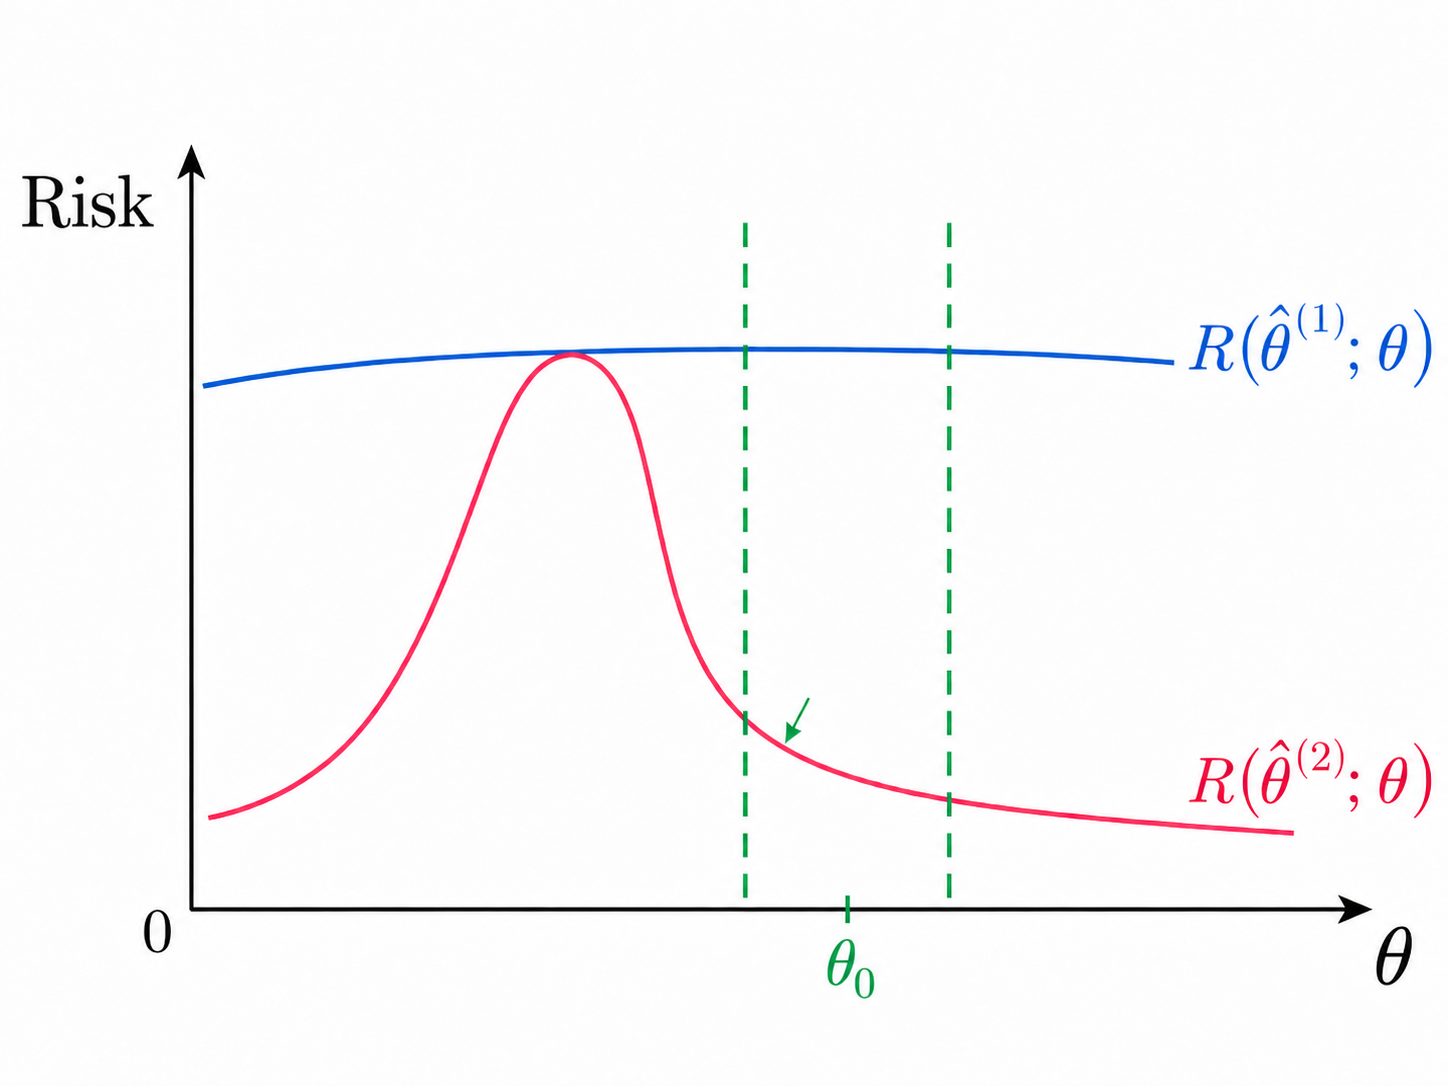
\includegraphics[width=0.78\textwidth]{./lec3-local-minimax-illustration.png}

  \small The dashed lines mark a local neighborhood of $\theta_0$. The local minimax criterion compares the largest risk within this neighborhood, rather than over the entire parameter space.
\end{center}

\end{document}
